\documentclass[../main.tex]{subfiles}
\begin{document}
\section{Systematic uncertainties}
\label{hh:sec:systematics}

\textcolor{red}{Intro to systematics}

\subsection*{Experimental uncertainties}

\subsubsection*{Luminosity}

The uncertainty in the measured integrated luminosity 
is obtained via dedicated Van-der-Meer scans and the stability of the detector response during data-taking \cite{lumi_1516}. It takes values of 1.2\%, 2.3\% and 2.5\% for the 2016 \cite{lumi_2016}, 2017 \cite{lumi_2017} and 2018 \cite{lumi_2018} datasets respectively. This uncertainties are partially correlated among the three years. These uncertainties are applied to all signals and to all backgrounds that are estimated fully from MC simulation. The normalizations of the $\text{t}\bar{\text{t}}$, $\text{Z}/\gamma^*+~$jets and QCD multi-jet processes is obtained from data, so this uncertainty is not applied.

\subsubsection*{Trigger scale factors}

Four uncertainties in the trigger scale factors are included to take into account the four different \tauh{} decay modules considered in the analysis. They are applied to the \tauh{} leg of each channel (both legs in the \tauh\tauh{} channel). Two additional uncertainties are used for the $\tau$ decays into an electron or a muon, while a final uncertainty is added in the \tauh\tauh{} channel in 2017 and 2018 to cover the jet legs scale factors of the VBF trigger.


\subsubsection*{Lepton reconstruction, isolation and identification}

Electron and muon reconstruction, isolation, and identification uncertainties are determined 
from the simulation-to-data scale factors; a value of 1~\% is obtained for both electrons and muons. An additional uncertainty of 3 (15)\% for $\tau$ leptons with $p_T< 100$~GeV ($p_T> 100$~GeV) is added in the \tauh\tauh{} decay channel.

\subsubsection*{L1 ECAL trigger prefiring}

The uncertainty on the correction factor used to account for the L1 prefiring is taken into account by varying the obtained weight by this uncertainty, resulting in the addition of a 2\% uncertainty in the final discriminant.

\subsubsection*{PU reweighting}

An uncertainty on the PU reweighting technique described in Section~\ref{hh:sec:pu} is estimated by varying the values of the applied PU weights by their uncertainty. The resulting systematic uncertainty is estimated to have a value of 1\%.

\subsubsection{PU jet identification}

Uncertainties in he PU jet identification scale factors are included as functions of the jet $p_T$ and $\eta$. These uncertainties are included in an event-by-event basis, not modifying the individual objects.

\subsubsection*{$\text{t}\bar{\text{t}}$ normalization}

The normalization of the $\text{t}\bar{\text{t}}$ background is taken from a fit to a $\text{t}\bar{\text{t}}$ enriched control region for each year, as shown in Section~\ref{hh:subs:tt}. The resulting systematic uncertainty is below 1\% for each year.

\subsubsection*{$\text{Z}/\gamma^*+~$jets normalization}

The normalization of the $\text{Z}/\gamma^*+~$jets background is taken from a fit to 18 $\text{Z}/\gamma^*+~$jets enriched control regions per year, as described in Section~\ref{hh:subs:dy}. The resulting uncertainties range from 0.1 to 60\% depending on the year and the control region considered.

\subsubsection*{QCD multi-jet}

The contribution from QCD multi-jet background is determined using the ABCD method as described in Section~\ref{hh:subs:qcd}. Assuming that the contribution of the QCD multi-jet background is constant in the four regions considered (A, B, C and D), three uncertainties can be defined, all uncorrelated across categories, $\tau\tau$ decay channels and years:
\begin{itemize}
\item \textbf{Shape uncertainty}: as shown in Section~\ref{hh:subs:qcd}, the QCD multi-jet background shape is extracted from the selection included in region C. However, an additional estimation could be obtained if, instead of taking the shape from region C and computing the factor $k$ as the ratio of the yields coming from regions B and D, the shape was taken from region B and the factor $k$ is computed as the ratio between regions C and D. In fact, as shown in Figs.~\ref{hh:fig:qcd_shape_from_c} and \ref{hh:fig:qcd_shape_from_b}, the data/background agreement is very comparable when considering these two strategies. Therefore, the QCD background shape used in the analysis will come from the average of the shapes from the two regions. The two alternative shapes (from C and B) will be considered as the up and down templates for the QCD shape uncertainty.
\item \textbf{Uncertainty on the yield correction factor}: the statistical uncertainty on the correction factor B/D is a normalization uncertainty defined as the sum in quadrature of the statistical uncertainties on the event yields in regions B and D. The value of this uncertainty ranges from 5\% to 100\% depending on the category, channel and year considered.
\item \textbf{Additional uncertainty}: this normalization uncertainty is added only in the cases where the C/D factor obtained using the standard QCD definition of the C and D regions does not agree within uncertainties with the weighted average of the four alternative C/D yield points defined in the first validation test for the QCD multi-jet background estimation. It follows the expression
\begin{equation}
\text{add\_unc} = \sqrt{\left(\frac{(\text{C/D})_{\text{standard}} - (\text{C/D})_{\text{average}}}{(\text{C/D})_{\text{standard}}} \right)^2 - \left(\frac{\Delta(\text{C/D})_{\text{standard}}}{(\text{C/D})_{\text{standard}}} \right)^2}.
\end{equation}
\end{itemize}


Table~\ref{hh:tab:qcd_und} shows the QCD normalization percentage relative uncertainty for all years, channels and categories considered. For each cell, the first number is the statistical uncertainty on the yield correction factor, 2while the second (if it appears) is the additional uncertainty as defined above. The cell is empty if no QCD could be estimated (as either regions B, C or D have negative yield). Note that the statistical
uncertainty for all the VBF subcategories in the same year and channel is the same, as it comes from the VBF inclusive category (described in Section~\ref{hh:sec:event_categorization}.


\begin{figure}[h!]
\begin{center}
\subfloat[Boosted]{\includegraphics[width=0.33\textwidth]{Images/qcd_tests/shapes/2018/boosted/DNNoutSM_kl_1__pg_plots__qcd__blinded__tautau_os_iso__stack}}
\subfloat[Resolved, 1 b-tag]{\includegraphics[width=0.33\textwidth]{Images/qcd_tests/shapes/2018/resolved_1b/DNNoutSM_kl_1__pg_plots__qcd__blinded__tautau_os_iso__stack}}
\subfloat[Resolved, 2 b-tag]{\includegraphics[width=0.33\textwidth]{Images/qcd_tests/shapes/2018/resolved_2b/DNNoutSM_kl_1__pg_plots__qcd__blinded__tautau_os_iso__stack}} \\
\subfloat[VBF subcat.]{\includegraphics[width=0.33\textwidth]{Images/qcd_tests/shapes/2018/vbf/DNNoutSM_kl_1_hh_vbf_sm_c2v_merged_mpp__pg_plots__qcd__blinded__tautau_os_iso__stack__binopt_opt}}
\subfloat[ggF subcat.]{\includegraphics[width=0.33\textwidth]{Images/qcd_tests/shapes/2018/vbf/DNNoutSM_kl_1_hh_ggf_merged_mpp__pg_plots__qcd__blinded__tautau_os_iso__stack__binopt_opt}}
\subfloat[$\text{t}\bar{\text{t}}$ subcat.]{\includegraphics[width=0.33\textwidth]{Images/qcd_tests/shapes/2018/vbf/DNNoutSM_kl_1_tt_merged_mpp__pg_plots__qcd__blinded__tautau_os_iso__stack__binopt_opt}} \\
\subfloat[$\text{t}\bar{\text{t}}$H subcat.]{\includegraphics[width=0.33\textwidth]{Images/qcd_tests/shapes/2018/vbf/DNNoutSM_kl_1_tth_merged_mpp__pg_plots__qcd__blinded__tautau_os_iso__stack__binopt_opt}}
\subfloat[DY subcat.]{\includegraphics[width=0.33\textwidth]{Images/qcd_tests/shapes/2018/vbf/DNNoutSM_kl_1_dy_merged_mpp__pg_plots__qcd__blinded__tautau_os_iso__stack__binopt_opt}}
\end{center}
\caption{DNN output distributions for the analysis categories in the signal region. QCD background is estimated from the ABCD method taking the shape from region C and the $k$ factor from B/D. \textcolor{red}{Unblinded results to be included.}}
\label{hh:fig:qcd_shape_from_c}
\end{figure}

\begin{figure}[h!]
\begin{center}
\subfloat[Boosted]{\includegraphics[width=0.33\textwidth]{Images/qcd_tests/shapes/2018/boosted/DNNoutSM_kl_1__pg_plots__qcd_from_ss_iso__blinded__tautau_os_iso__stack}}
\subfloat[Resolved, 1 b-tag]{\includegraphics[width=0.33\textwidth]{Images/qcd_tests/shapes/2018/resolved_1b/DNNoutSM_kl_1__pg_plots__qcd_from_ss_iso__blinded__tautau_os_iso__stack}}
\subfloat[Resolved, 2 b-tag]{\includegraphics[width=0.33\textwidth]{Images/qcd_tests/shapes/2018/resolved_2b/DNNoutSM_kl_1__pg_plots__qcd_from_ss_iso__blinded__tautau_os_iso__stack}}\\
\subfloat[VBF subcat.]{\includegraphics[width=0.33\textwidth]{Images/qcd_tests/shapes/2018/vbf/DNNoutSM_kl_1_hh_vbf_sm_c2v_merged_mpp__pg_plots__qcd_from_ss_iso__blinded__tautau_os_iso__stack__binopt_opt}}
\subfloat[ggF subcat.]{\includegraphics[width=0.33\textwidth]{Images/qcd_tests/shapes/2018/vbf/DNNoutSM_kl_1_hh_ggf_merged_mpp__pg_plots__qcd_from_ss_iso__blinded__tautau_os_iso__stack__binopt_opt}}
\subfloat[$\text{t}\bar{\text{t}}$ subcat.]{\includegraphics[width=0.33\textwidth]{Images/qcd_tests/shapes/2018/vbf/DNNoutSM_kl_1_tt_merged_mpp__pg_plots__qcd_from_ss_iso__blinded__tautau_os_iso__stack__binopt_opt}}\\
\subfloat[$\text{t}\bar{\text{t}}$H subcat.]{\includegraphics[width=0.33\textwidth]{Images/qcd_tests/shapes/2018/vbf/DNNoutSM_kl_1_tth_merged_mpp__pg_plots__qcd_from_ss_iso__blinded__tautau_os_iso__stack__binopt_opt}}
\subfloat[DY subcat.]{\includegraphics[width=0.33\textwidth]{Images/qcd_tests/shapes/2018/vbf/DNNoutSM_kl_1_dy_merged_mpp__pg_plots__qcd_from_ss_iso__blinded__tautau_os_iso__stack__binopt_opt}}
\end{center}
\caption{DNN output distributions for the analysis categories in the signal region. QCD background is estimated from the ABCD method taking the shape from region B and the $k$ factor from C/D. \textcolor{red}{Unblinded results to be included.}}
\label{hh:fig:qcd_shape_from_b}
\end{figure}


\begin{table}[!h]
  \begin{center}
    \begin{tabular}{c | c | c | c | c}
                                        &                  & 2016         & 2017         & 2018         \\\hline
                                        & $\tau_h\tau_h$   & 198.0        & 44.5         & 60.6         \\
    Boosted                             & $\tau_\mu\tau_h$ & $-$          & $-$          & $-$          \\
                                        & $\tau_e\tau_h$   & $-$          & $-$          & $-$          \\
    \hline
                                        & $\tau_h\tau_h$   & 7.6          & 5.9          & 4.7          \\
    Resolved, 1 b-tag                        & $\tau_\mu\tau_h$ & 7.1          & 7.4          & 13.6         \\
                                        & $\tau_e\tau_h$   & 14.8         & 10.0         & 10.0         \\
    \hline
                                        & $\tau_h\tau_h$   & 118.5        & 21.9         & 21.6         \\
    Resolved, 2 b-tag                       & $\tau_\mu\tau_h$ & 18.6         & 17.7         & 10.8         \\
                                        & $\tau_e\tau_h$   & 42.8         & $-$          & $-$          \\
    \hline
                                        & $\tau_h\tau_h$   & 27.2         & 23.2         & 14.1         \\
    VBF subcategory         & $\tau_\mu\tau_h$ & 81.7         & 26.7 , 36.2  & 11.6         \\
                                        & $\tau_e\tau_h$   & 122.0        & 33.1         & $-$          \\
    \hline
                                        & $\tau_h\tau_h$   & 27.2         & 23.2         & 14.1         \\
    ggF subcategory                     & $\tau_\mu\tau_h$ & $-$          & $-$          & 11.6         \\
                                        & $\tau_e\tau_h$   & $-$          & $-$          & $-$          \\
    \hline
                                        & $\tau_h\tau_h$   & 27.2         & 23.2         & 14.1         \\
    $\text{t}\bar{\text{t}}$ subcategory& $\tau_\mu\tau_h$ & $-$          & $-$          & 11.6         \\
                                        & $\tau_e\tau_h$   & $-$          & $-$          & 25.7         \\
    \hline
                                        & $\tau_h\tau_h$   & $-$          & 23.2         & 14.1         \\
    $\text{t}\bar{\text{t}}$H subcategory                    & $\tau_\mu\tau_h$ & 81.7         & $-$          & $-$          \\
                                        & $\tau_e\tau_h$   & $-$          & $-$          & $-$          \\
    \hline
                                        & $\tau_h\tau_h$   & 27.2         & 23.2         & 14.1         \\
    DY subcategory                     & $\tau_\mu\tau_h$ & 81.7 , 81.2  & 26.7         & 11.6 , 7.7   \\
                                        & $\tau_e\tau_h$   & $-$          & $-$          & 25.7         \\
     \hline
    \end{tabular}
  \end{center}
    \caption{QCD normalization percentage relative uncertainty. For each cell, the first number is the statistical uncertainty on the yield correction factor, while the second (if it appears) is the additional uncertainty.
    The cell is empty if no QCD could be estimated (as either regions B, C or D have negative yield). Note that the statistical uncertainty for all the VBF subcategories in the same year and channel is the same, as it comes from the VBF inclusive category.}
	\label{hh:tab:qcd_unc}
\end{table}

\subsubsection*{\tauh{} energy scale}

The uncertainty on the measurement of the energy of the $\tau$ leptons decaying into hadrons can lead to a change in the distribution of the discriminant variables. An uncertainty on the energy scale of each \tauh{} is derived by combining low- and high-$p_T$ measurements in Z$\to\tau\tau$ and $\text{W}^*\to\tau\nu$ events. Four different uncertainties are included, one for each \tauh{} decay mode considered in the analysis. Each uncertainty only applies to the \tauh{} reconstructed with the specific decay mode, the other remain unchanged.

\subsubsection*{Energy scale of electrons and muons misidentified as \tauh{}}

Separate uncertainties in the energy scale of electrons misidentified as \tauh{} candidates are provided to take into account the h${}^\pm$ and h${}^\pm\pi^0$.

For the muons misidentified as \tauh{} candidates, the uncertainty in the energy scale is 1\%, uncorrelated across decay modes.

\subsubsection*{Jets faking \tauh}

Uncertainties coming from the misidentification of jets as \tauh{} candidates are estimated with a new control region in the \taumu\tauh{} channel defined by inverting the charge requirement on the $\tau\tau$ pair and imposing that neither of the b jet candidates pass the medium DeepJet working point. Two uncorrelated uncertainties are derived per year, one for the barrel and another one for the endcap, taking values from 11 to 28\% depending on the year and region.

\subsubsection*{Jet energy scale and resolution}

Several uncertainties related to the calibration of the jet energy scale (JES) and resolution (JER) are included. For JES, 11 separate sources are included per year. The ones common between years are treated as fully correlated, while the ones appearing only in one year are left as uncorrelated. For JER, the energy of the simulated jets is smeared in order to match the observed energy resolution in data, as shown in Section~\ref{hh:sec:corrections}. An uncertainty on the JER correction factor is provided in different regions of $\eta$ and $p_T$ for each year, resulting in a shift in the final distributions.


\subsubsection*{DeepTau identification}

Several uncertainties coming from the application of the different DeepTau identification scale factors is determined by using a tag-and-probe procedure as a function of the \tauh{} candidate $p_T$. For the identification of \tauh{} against jets, five uncertainties are provided, binned between 20 and 25 GeV, 25 and 30 GeV, 30 and 35 GeV, 35 and 40 GeV, and from 40 GeV onwards. For the \taue\tauh and \taumu\tauh channels, 




\subsubsection*{b-tagging efficiency}

The uncertainties included in the b-tagging efficiency cover both the contamination from udscg (cb) jets in heavy- (light-) flavor regions and the statistical fluctuations in the data and simulation samples used for the computation of the efficiency. Some of the uncertainties are correlated across all years, while all of them modify the overall weight of each event, not the individual objects.


\subsection*{Theoretical uncertainties}

\subsubsection*{HH production cross section}

The theoretical uncertainty in the cross section HH production via ggF is ${}^{+6\%}_{-23\%}$ (scale + $m_t$) $\pm 3\%$ (PDF + $\alpha_s$)~fb \cite{hh:results:ggf_xs} and via VBF ${}^{+0.03\%}_{-0.04\%}$ (scale) $\pm 2.1\%$ (PDF + $\alpha_s$) \cite{hh:results:vbf_xs}. These uncertainties are only considered when upper limits are obtained with respect to the SM value, not in the upper limits on the cross section.

\subsubsection*{H branching fractions}

Two uncertainties are included to account for the Higgs boson decay \cite{hh:results:h_bf} into bb and $\tau\tau$: $\pm 0.65\%$ (theory) ${}^{+0.72\%}_{-0.74\%}$ ($m_q$) ${}^{+0.78\%}_{-0.80\%}$ ($\alpha_s$) and 
${}^{+1.16\%}_{-1.17\%}$  (theory) ${}^{-0.98\%}_{-0.99\%}$ ($m_q$) $\pm 0.62\%$ ($\alpha_s$) respectively, where $m_q$ stands for the quark mass. As in the HH production cross section uncertainties, these are only included when computing the limit with respect to the SM expectation.

\subsubsection*{Background cross sections}

For the processes modelled exclusively from simulated events, several uncertainties are included, varying from 0.4 to 10\% (\textcolor{red}{Worth showing a table with names and numbers?}).


\subsubsection*{VBF dipole recoil uncertainty}

The default CMS showering Pythia8 configuration used in the standard MC production does not provide a good modelling of the third leading jet distribution for the VBF signal \cite{hh:results:dipole_recoil}. This can be improved by setting the dipole recoil option, available in recent Pythia8 versions, to ON. Alternative VBF signal samples with \kvv=1 and \kvv=2 (with the additional couplings set to the SM expectation) were produced for 2017 and 2018 using this alternative option, and have been used to compute a normalization systematic uncertainty to the standard VBF signal samples due to this effect.

The uncertainty is computed per category, channel and year taking the most conservative value between the ratio of integrated yields in the dipole recoil ON/OFF samples augmented by its statistical uncertainty and the ratio in normalised per bin yields in the corresponding DNN distributions, where the yield per DNN bin has been normalized by the yield in the highest statistics bin in the standard VBF sample with dipole recoil OFF. An example of these computations is shown in Fig.~\ref{hh:fig:dipole_recoil} for the 2018 samples with \kvv=1 in the VBF subcategory.

\begin{figure}[h!]
\begin{center}
\subfloat{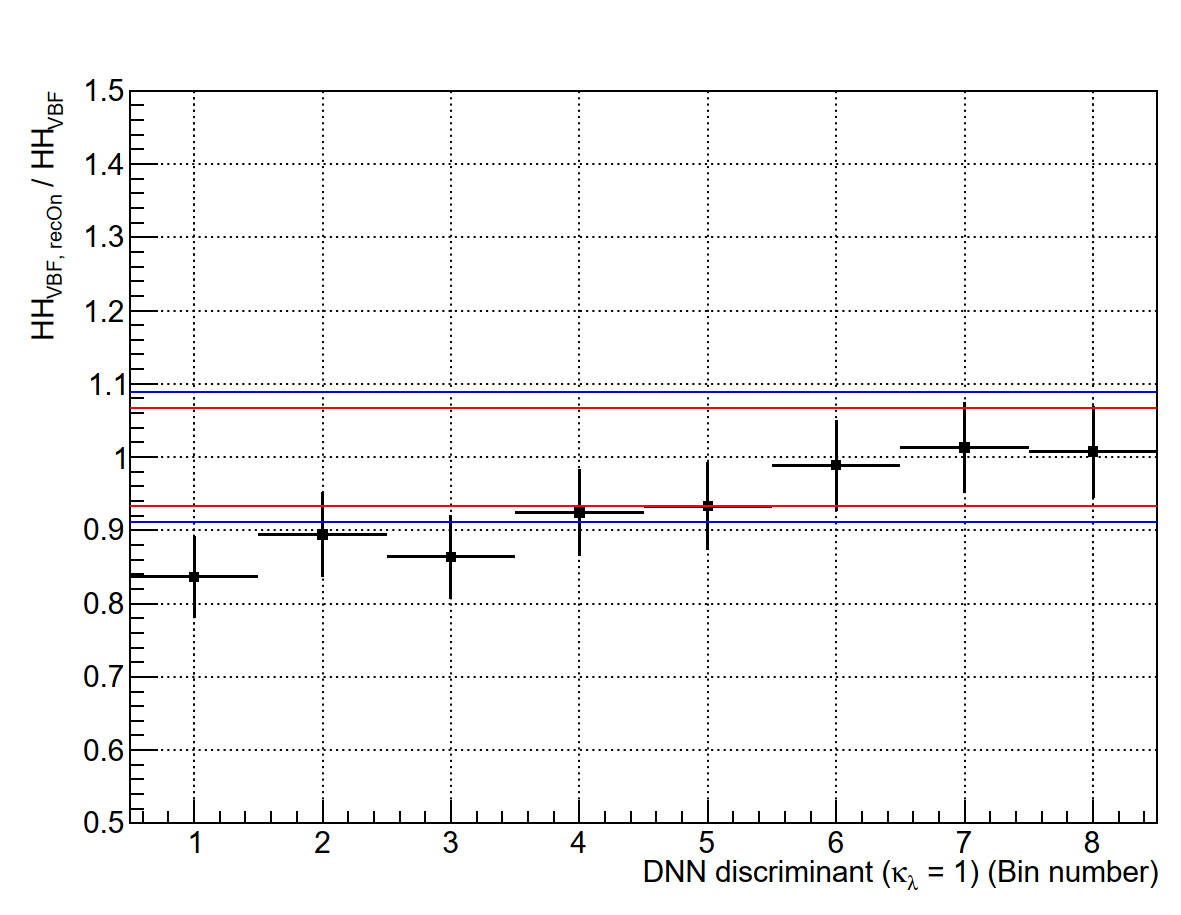
\includegraphics[width=0.49\textwidth]{Images/vbf_dipole_mean}}
\subfloat{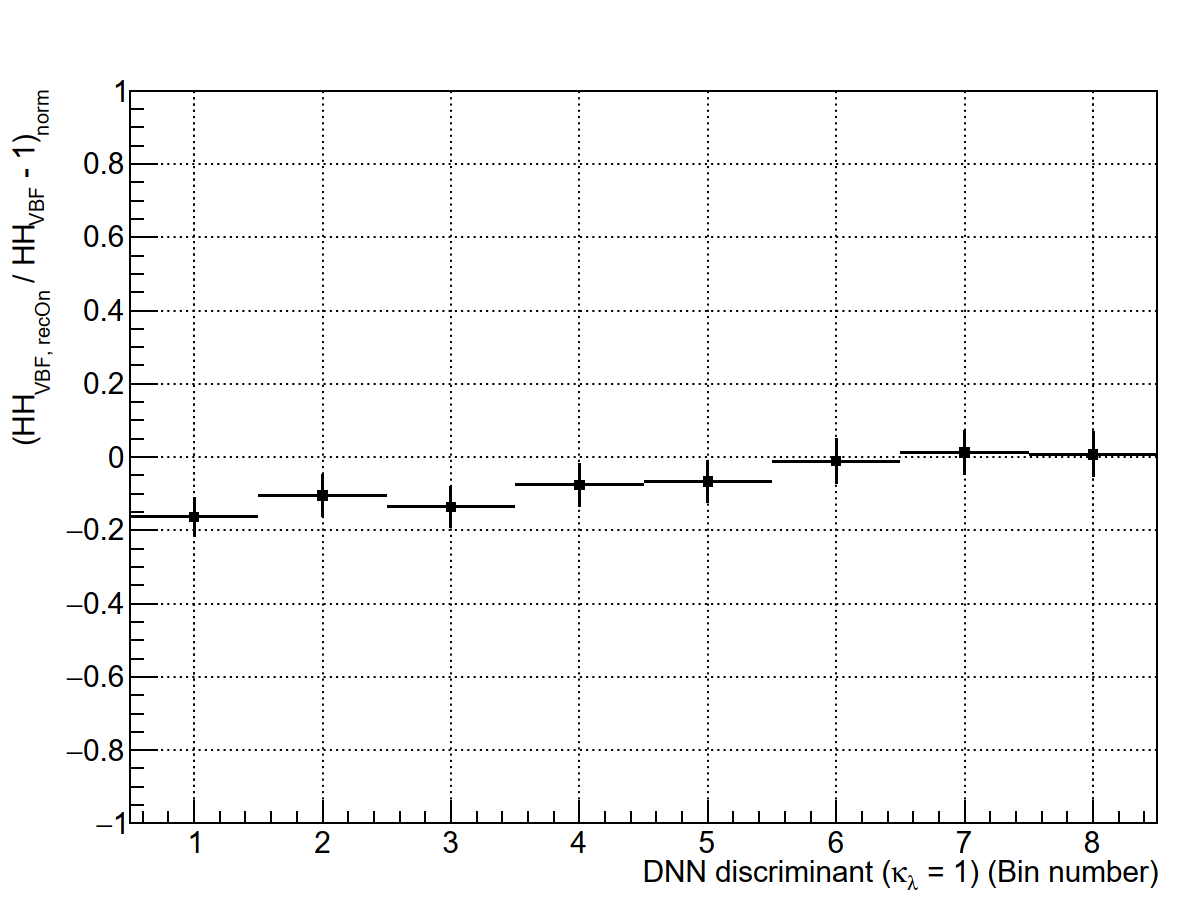
\includegraphics[width=0.49\textwidth]{Images/vbf_dipole_norm}}
\end{center}
\caption{Dipole recoil ON/OFF uncertainty tests for the 2018 VBF samples with \kvv=1 in the VBF subcategory. Left: Ratio between the DNN distributions. Red lines show the ratio of integrated yields and its symmetric with respect to 1 and blue lines after augmenting this ratio by the statistical uncertainty. The dipole recoil uncertainty (up and down templates) derived from this plot is taken by substracting 1 to the blue lines. Right: Ratio between the DNN distributions after normalizing by the yield in the bin with the highest statistics. The uncertainty derived from this plot is taken from the bin with the highest contribution in absolute value and its opposite.}
\label{hh:fig:dipole_recoil}
\end{figure}


The final uncertainty has been set to be the same for all six VBF processes used in the signal modelling in all years for each category and channel by taking the most conservative value between 2017 and 2017 and both \kvv values. The uncertainty can be seen in Table~\ref{hh:tab:dipole_recoil} and is considered as correlated between years and categories, but uncorrelated between the three channels.

\begin{table}[h!]
\begin{center}
\begin{tabular}{c | c  c c}
Category / Channel                     & \taue\tauh & \taumu\tauh & \tauh\tauh \\\hline
Boosted                                & 20.4        & 39.3       & 19.8 \\
Resolved, 1 b-tag                      & 14.5        & 11.8       & 21.9 \\
Resolved, 2 b-tag                      & 26.9        & 15.4       & 17.1 \\
VBF subcategory   					   & 16.3        & 18.7       &  9.0 \\
ggF subcategory                        & 55.2        & 50.4       & 33.7 \\
$\text{t}\bar{\text{t}}$ subcategory   & 42.0        & 41.7       & 56.7 \\
$\text{t}\bar{\text{t}}$H  subcategory & 67.2        & 69.6       & 70.5 \\
DY subcategory                         & 46.7        & 48.3       & 52.3 \\
\end{tabular}
\end{center}
\caption{VBF dipole recoil uncertainty values in \%.}
\label{hh:tab:dipole_recoil}
\end{table}







\end{document}

